\documentclass{ouexam}

\usepackage{graphicx}
\usepackage{listings}

\examyear{2001}
\department{Information Science}
\papernumber{INFO 321}
\papertitle{Database Systems}
\instructions{Answer \underline{ALL} questions.}
\allowcalculators[approved]

\begin{document}

\lstloadlanguages{ODL,OQL,[Oracle8]SQL,[Oracle8]PLSQL}
\lstset%
{	basicstyle=\sffamily,
	showstringspaces=false,
	tabsize=2,
	xleftmargin=1cm,
	belowskip=0pt,
	commentstyle=\itshape,
	numbers=left,
	numberstyle=\scriptsize,
	numbersep=5pt,
	columns=fullflexible,
}

\maketitlepage


%======================================================================
% PHYSICAL TUNING SECTION
%======================================================================
\begin{examsection}{25}{}{Questions in this section (total 25 marks) relate to
physical database design and tuning.}

%======================================================================

\begin{question}{10}

	A major U.S. mail order firm is having performance problems with queries on
	the \textsf{Customer} table in its Oracle8 order-processing database.
	Consider the following information about the \textsf{Customer} table, then
	answer the questions below:	\\

	\textsf{\textbf{Customer}(\underline{customer\_no}, name, address, city,
	state, country, phone, email, status)}

	\begin{itemize}

		\item \textsf{customer\_no} is the primary key and because this is an
		Oracle8 database, a unique B-tree index has been automatically created
		on this column.

		\item \textsf{status} is a single character column that holds one of
		the values `I' (inactive), `B' (bronze), `S' (silver) or `G' (gold).
		The value of this column is determined by a customer's order history.

		\item About 10\% of customers are inactive, about 50\% have bronze
		status, about 35\% have silver status and about 5\% have gold status.

		\item The average row size is about 200 bytes and there are
		approximately 5,000,000 rows.

		\item The \textsf{Customer} table is heavily queried (averaging thirty
		new queries per minute) by four different groups of employees. Group~1
		queries only inactive customers, group~2 queries only bronze status
		customers and groups~3 and~4 both query only silver and gold status
		customers. Members of any group may query the table at any time and
		queries often overlap.

		\item UPDATE, INSERT and DELETE operations on the table are uncommon.

		\item Very few queries are for individual customers; rather, most
		queries are based on various combinations of values from
		\textsf{status}, \textsf{city}, \textsf{state} and \textsf{country}.

	\end{itemize}
	\medskip

%----------------------------------------------------------------------

	\begin{subquestion}{3}
		Describe and justify an \emph{index-based} physical tuning solution
		that will improve the performance of queries on the \textsf{Customer}
		table. (No code is required.)
		\begin{marking}
			Since queries tend to be on combinations of several low-cardinality
			columns [1] and the table is very large [1], the most effective
			solution would be to place bitmap indexes on status, city, state
			and country [1].

			B-tree indexes on any of the individual columns would not be ideal
			because of their low cardinality. A possible alternative is a
			composite B-tree index on all four columns [1 for suggesting this
			if appropriate], but this is not ideal and would be much larger
			than the four bitmap indexes [1 for this explanation if
			appropriate].

			Hashing is definitely \emph{not} an option, because very few
			queries are exact match.
		\end{marking}
	\end{subquestion}
		
%----------------------------------------------------------------------

	\begin{subquestion}{7}
		\begin{subsubquestion}{5}
			\label{nonindex}
			Assuming that there are two identical fast disks available,
			describe and justify two alternative \emph{non index-based}
			physical tuning solutions that will improve the performance of
			queries on the \textsf{Customer} table. For each solution include
			details of how the two disks will be used. (No code is required.)
			\begin{marking}
				Alternative 1: partition the table across the two disks based
				on status (four partitions, one for each status value) [1].
				This will allow simultaneous parallel access to different parts
				of the table by the different groups [1]. Since two groups both
				access silver and gold customers, it makes sense to put the
				silver customers on disk one and the gold customers on disk
				two. Bronze customers account for 50\% of the table, so it
				makes sense to also put them on disk two (as the gold customers
				are the smallest group), and put the inactive customers on disk
				one with the silver customers. [1 for any sensible partitioning
				scheme]
	
				Alternative 2: replicate the table across both disks (one
				replica on each disk) [1]. This will also provide simultaneous
				parallel access to the data (hard to tell whether this would be
				better or worse than the partitioning above) [1].
	
				Note that any solution must be capable of being implemented in
				Oracle8.
			\end{marking}
		\end{subsubquestion}

		\begin{subsubquestion}{2}
			Briefly discuss the relative advantages and/or disadvantages of the
			two alternative solutions you described in part~\ref{nonindex}
			above.
			\begin{marking}
				The partitioning solution given above doesn't really help with
				the bronze customer rows---we would need random horizontal
				partitioning to really help with this, which Oracle8 doesn't
				support. More generally, Oracle8 does not migrate rows into the
				correct partition if a customer's status changes, so the data
				will need to be reloaded occasionally [1].

				For replication, we have the usual problem of keeping the
				replicas synchronised if they are both read/write. This is
				somewhat mitigated by the fact that there are only two copies
				[1].
			\end{marking}
		\end{subsubquestion}
	\end{subquestion}
	
%----------------------------------------------------------------------

\end{question}


\newpage

%======================================================================

\begin{question}{10}
	There are two generic parameters that affect the structure of a B-tree
	index.

%----------------------------------------------------------------------

	\begin{subquestion}{6}
		Identify these two parameters and describe what each parameter
		specifies. Use diagrams to illustrate your answer.
		\begin{marking}
			\emph{Node size} [1] specifies the maximum number of pointers in
			each index node [1]. Suitable diagram [1].

			\emph{Percentage fill} [1] specifies the number of pointers in each
			index node that are allocated when a node is created [1]. In
			effect, it determines the amount of free space left in each node.
			Suitable diagram [1].
		\end{marking}
	\end{subquestion}
	
%----------------------------------------------------------------------

	\begin{subquestion}{4}
		For each of the two parameters, discuss the practical effect(s) of:
		\begin{subsubquestion}{2}
			high values of the parameter; and
			\begin{marking}
				Large node size reduces the height of the B-tree, resulting in
				potentially fewer I/Os to access a leaf node [$\frac{1}{2}$].
				It can however increase the number of rows locked in a single
				leaf node [$\frac{1}{2}$].
	
				High percent fill means that most pointers in a node will be
				allocated when the node is created [$\frac{1}{2}$]. This leaves
				little free space in the B-tree for new key values or key
				values that change [$\frac{1}{2}$].
			\end{marking}
		\end{subsubquestion}
		\begin{subsubquestion}{2}
			low values of the parameter.
			\begin{marking}
				Small node size increases the height of the B-tree, resulting
				in potentially more I/Os to access a leaf node [$\frac{1}{2}$].
				The number of rows locked in a single leaf node will be reduced
				[$\frac{1}{2}$].
	
				Low percent fill means that most pointers in a node will not be
				allocated when the node is created [$\frac{1}{2}$]. This leaves
				little free space in the B-tree for new key values or key
				values that change [$\frac{1}{2}$].
			\end{marking}
		\end{subsubquestion}
	\end{subquestion}
	
%----------------------------------------------------------------------

\end{question}
	
%======================================================================

\begin{question}{5}\label{clusterq}

%----------------------------------------------------------------------

	\begin{subquestion}{2}
		Define what is meant by the term ``clustering'' in the context of
		physical database design and tuning, and explain why it is beneficial.
		\begin{marking}
			Clustering is the grouping of related rows physically near to each
			other on disk [1] so that they may be retrieved in as few I/Os as
			possible (ideally one)---beneficial because of the slowness of disk
			I/O compared to memory I/O [1].
		\end{marking}
	\end{subquestion}
	
%----------------------------------------------------------------------

	\begin{subquestion}{3}\label{clusterqcode}
		Consider the following Oracle8 SQL table definition:
		
		\begin{lstlisting}[language={[Oracle8]SQL}]{}
create table enrolment
(	student_id char(7),
	paper_code char(7),
	enrol_year number(4),
  
	primary key (student_id, paper_code, enrol_year)
);
		\end{lstlisting}

		The \textsf{Enrolment} table is often queried for all rows relating to
		a particular student in a particular year (for example, student 1234567
		in 1998, student 9876543 in 2000, etc.). Write appropriate Oracle8 SQL
		code that will cluster the rows of the table in such a way as to
		support these types of query (you do not need to calculate cluster
		sizes). Relevant Oracle8 syntax diagrams are given on the next page.
		\begin{marking}
			\begin{lstlisting}[language={[Oracle8]SQL}]{}
create cluster enrolment_cluster (student_id char(7), year number(4));

create index enrol_cluster_index on cluster enrolment_cluster;

create table enrolment
(	student_id char(7),
	paper_code char(7),
	enrol_year number(4),
  
	primary key (student_id, paper_code, enrol_year)
) cluster enrolment_cluster(student_id, enrol_year);
			\end{lstlisting}
		\end{marking}
		[1] each for correct cluster, cluster index and table clustering.
	\end{subquestion}

\end{question}


\end{examsection}


\newpage


% CREATE CLUSTER (first part), p 4-207

\begin{center}
	\textbf{Oracle8 syntax diagrams for use in
	question~\ref{clusterq}(\ref{clusterqcode})}
	
	\bigskip

	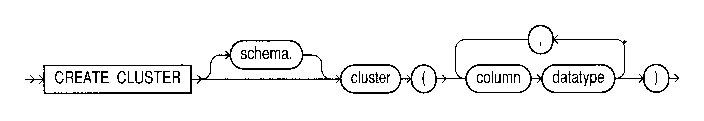
\includegraphics{CreateCluster}

	\vfill

% CREATE INDEX (parts 1 and 2), p. 4-238

	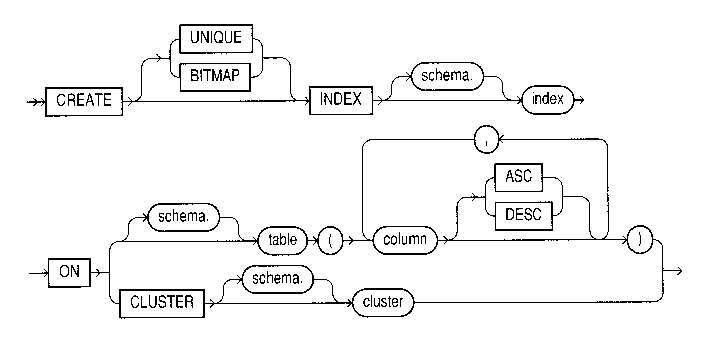
\includegraphics{CreateIndex}

% CREATE TABLE (parts 1 and 2), p. 4-308

	\vfill

	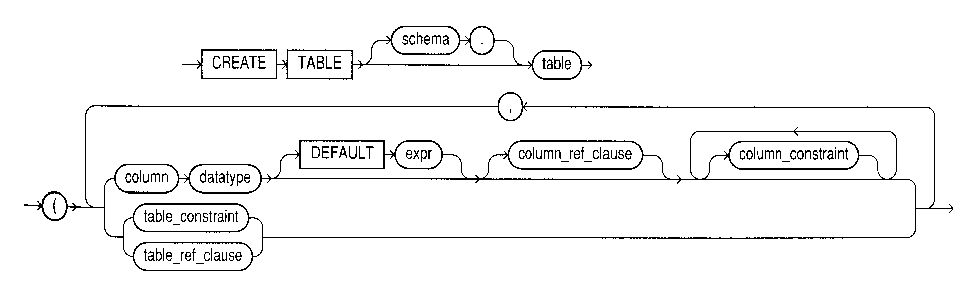
\includegraphics{CreateTable1}
	
	\bigskip	
	
	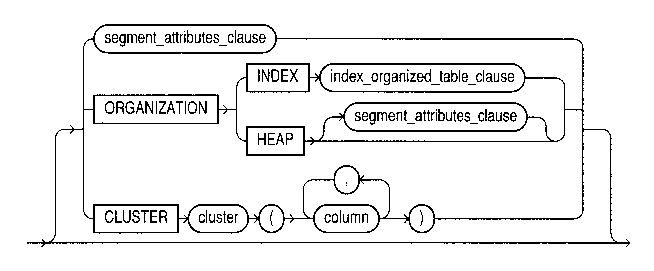
\includegraphics{CreateTable2}
\end{center}

%======================================================================
% OBJECT DBMS SECTION
%======================================================================
\begin{examsection}{25}{}{Questions in this section (total 25 marks) relate to object
database management systems and the Object Data Management Group's object model
(ODMG 3.0).}

%======================================================================

\begin{question}{10}\label{odlq}
	Examine the following Object Definition Language (ODL) schema, then answer
	the questions below.

	\begin{lstlisting}[language=ODL]{}
module ExamODL
{
	interface Person
	{
		attribute string name;
		attribute date birth_date;
		attribute struct Address
		{	string street;
			string city;
			string country;
		} home_address;
	};

	class Employee : Person (extent Staff key emp_ID)
	{
		attribute string emp_ID;
		attribute string position;
		attribute string department;
		attribute unsigned long salary;
	};
};
	\end{lstlisting}
	
%----------------------------------------------------------------------

	\begin{subquestion}{2}
		How many attributes will instances of the \textsf{Employee} class have?
		Explain your answer.
		\begin{marking}
			This depends on your interpretation of what constitutes an
			attribute. I prefer seven [1]. It has four of its own and three
			inherited from the \textsf{Person} class (\textsf{home\_address}
			being counted as a single embedded literal attribute) [1].

			Nine is a possible alternative answer [1], because you could count
			\textsf{home\_address} as three attributes, giving four local and
			five inherited attributes [1].

			No marks for any other number \emph{unless} it has a sensible
			explanation, in which case award marks as appropriate.
		\end{marking}
	\end{subquestion}
	
%----------------------------------------------------------------------

	\begin{subquestion}{3}
		Examine the clause
		``\lstinline[language={[Oracle8]SQL}]+(extent Staff key emp_ID)+''
		on line 14 of the ODL listing above.

		\begin{subsubquestion}{2}
			Explain the effect(s) of this clause.
			\begin{marking}
				\lstinline[language={[Oracle8]SQL}]+extent Staff+ defines the
				name of the \emph{extent} (collection of all instances) of the
				\textsf{Employee} class [1].

				\lstinline[language={[Oracle8]SQL}]+key emp_ID+ defines
				\textsf{emp\_ID} to be an \emph{object key} for the
				\textsf{Employee} class [1].
			\end{marking}
		\end{subsubquestion}
		
		\begin{subsubquestion}{1}
			Identify the relational equivalents of the items specified in this
			clause.
			\begin{marking}
				Extent = relation [$\frac{1}{2}$] and object key = primary key
				[$\frac{1}{2}$].
			\end{marking}
		\end{subsubquestion}
	\end{subquestion}	

%----------------------------------------------------------------------

	\begin{subquestion}{5}\label{oracleodl}
		Write \emph{all} the code required to implement an Oracle8 object type
		that is as similar as possible to the \textsf{Employee} class. The
		syntax diagram for the \textsf{\textbf{create type}} statement is given
		on the next page.
		\begin{marking}
			\begin{lstlisting}[language={[Oracle8]SQL}]{}
create type address_type as object
(	street varchar2(50),	-- the data types aren't that important
	city varchar2(30),		-- as long as they roughly match
	country varchar2(30)
);

create type employee_type as object
(	emp_id char(7),
	name varchar2(50),
	birth_date date,
	home_address address_type,
	position char(10),
	department char(20),
	salary number
);
			\end{lstlisting}
			[--1] for major errors, or for not including \textsf{address\_type}
			as a separate object type. [--$\frac{1}{2}$] for each attribute
			missing or in the wrong place.
		\end{marking}
	\end{subquestion}
	
\end{question}

\newpage

\begin{center}
	\textbf{Oracle8 syntax diagram for use in
	question~\ref{odlq}(\ref{oracleodl})}
	
	\bigskip
	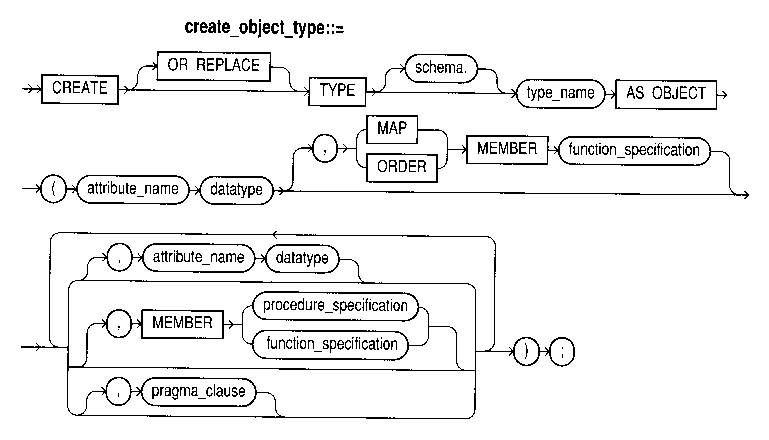
\includegraphics{CreateObjectType}
	\bigskip\bigskip
\end{center}

%======================================================================

\begin{question}{15}

%----------------------------------------------------------------------

	\begin{subquestion}{4}
		Compare in detail the ODMG concept of an \emph{object name} with the
		relational concept of a \emph{primary key}.
		\begin{marking}
			An object name is a meaningful user-generated identifier
			[$\frac{1}{2}$] for a single, specific object instance
			[$\frac{1}{2}$]. It is not part of the object's state
			[$\frac{1}{2}$] and a particular instance can have multiple object
			names associated with it [$\frac{1}{2}$].

			In comparison, a primary key is also user-defined (but may not
			always be meaningful) [$\frac{1}{2}$]. While a primary key uniquely
			identifies individual rows (which are the equivalents of object
			instances), it is associated with \emph{all} rows in a table, not
			just a single row [$\frac{1}{2}$]. A primary key comprises
			attributes of the relation, so it is part of the relation's
			``state'' [$\frac{1}{2}$]. An individual row has only one primary
			key associated with it [$\frac{1}{2}$].
		\end{marking}
	\end{subquestion}
	
%----------------------------------------------------------------------

	\begin{subquestion}{4}
		Compare in detail the ODMG concept of a \emph{relationship} with the
		relational concept of a \emph{foreign key}, with particular emphasis on
		any differences between the two concepts. Use an appropriate diagram or
		diagrams to illustrate your answer.
		\begin{marking}
			An ODMG relationship is a binary association between two object
			type, comprising a pair of \emph{traversal paths}, which are
			effectively pointers linking the two related instances [1]. ODMG
			relationships may be one-to-one, one-to-many or many-to-many, but
			we cannot specify participation [1].

			A relational foreign key is also a binary association between two
			relations, comprising an attribute stored in one of the relations
			that refers to the primary key of the other relation; in this
			respect, it is really equivalent to a traversal path rather than a
			full ODMG relationship [1]. Relationships defined by foreign keys
			cannot be many-to-many, but we can partially specify participation
			[1].

			Useful diagram(s).
		\end{marking}
	\end{subquestion}
	
%----------------------------------------------------------------------

	\begin{subquestion}{6}
		Define in detail the ODMG concepts of \emph{interface}, \emph{class}
		and \emph{literal}.
		\begin{marking}
			An interface is an ODMG object type that defines behaviour only
			[1]. You cannot create instances of interfaces (cf. abstract
			classes) [1].

			A class is an ODMG object type that can define both state and
			behaviour [1]. You can create instances of classes [1].

			A literal is an ODMG type (non-object) that defines state only [1].
			They have no identity and are effectively just structured data
			types [1].
		\end{marking}
	\end{subquestion}
	
%----------------------------------------------------------------------

	\begin{subquestion}{1}
		Date and Darwen claim in their \emph{Third Manifesto} that the
		relational model can support objects if it is implemented correctly.
		Briefly explain how they claim this can be achieved.
		\begin{marking}
			If we implement domains correctly/fully then they are effectively
			the equivalent of an object class [1].
		\end{marking}
	\end{subquestion}

\end{question}


\end{examsection}


%======================================================================
% DISTRIBUTED DBMS SECTION
%======================================================================
\begin{examsection}{25}{}{Questions in this section (total 25 marks) relate to
distributed database systems.}

%======================================================================

\begin{question}{4}
	Describe what is meant by the terms ``distributed data'' and ``distributed
	database'' and explain the key difference(s) between the two. Use an
	example to illustrate the difference(s).
	\begin{marking}
		Distributed data are spread across multiple nodes on a network but are
		neither centrally managed nor highly integrated [1]. A distributed
		database combines distributed data with distributed database processing
		[1] (including management, access and transaction processing)---this is
		the key difference [1]. Reasonable example [1].
	\end{marking}
\end{question}

%======================================================================

\begin{question}{10}
	Date's ``objective zero'' for distributed database management systems
	states ``a distributed database looks and behaves like a non-distributed
	database to any user''. Describe two \emph{different} ways in which this
	objective may be achieved, and for each discuss in detail how well it is
	implemented in Oracle8.
	\begin{marking}
		Basically a detailed description of any two of Date's objectives.
		Example: Location transparency is the ability to query data without
		needing to know on which network node the data are physically located.
		It is implemented reasonably well in Oracle8 by way of synonyms and
		views, after some initial setup work. [2 marks for description, 3 marks
		for implementation]
	\end{marking}
\end{question}

%======================================================================

\begin{question}{5}
	A company currently has a distributed database spread across two sites. It
	is necessary to move some data from one site to the other.

%----------------------------------------------------------------------

	\begin{subquestion}{3}
		Describe the general process that allows us to complete distributed
		transactions such as that described above with reasonable safety.
		\begin{marking}
			This is a distributed transaction, so the process involved is
			two-phase commit. In the first (\emph{prepare}) phase, the
			transaction coordinator tells all sites involved in the transaction
			to prepare to commit (by flushing buffers, locking data, etc.).
			Each site then responds ``OK'' or ``abort''. In the second
			(\emph{commit}) phase, if all sites respond ``OK'' the coordinator
			tells all sites to commit, otherwise it tells all sites to roll
			back.

			[1] for identifying 2PC, [1] each for both phases.
		\end{marking}
	\end{subquestion}
	
%----------------------------------------------------------------------

	\begin{subquestion}{2}
		Assuming an Oracle8 distributed database, give an example of a
		situation in which it may not be possible to automatically recover from
		a failed distributed transaction, and explain how such a situation
		might be dealt with.
		\begin{marking}
			If a site fails for a short period, in-doubt transactions will
			automatically complete when the site comes back up. If however the
			outage is for a significant period of time, then the DBMS cannot
			automatically commit in-doubt transactions as the data context may
			have changed considerably in the interim [1]. The DBA can commit or
			roll back in-doubt transactions manually, but this is risky [1].
		\end{marking} 
	\end{subquestion}

\end{question}

%======================================================================

\begin{question}{6}

%----------------------------------------------------------------------

	\begin{subquestion}{2}
		Consider the following Oracle8 SQL statement:
		\begin{lstlisting}[language={[Oracle8]SQL},numbers=none]{}
create synonym exam_synonym for sales.customer@db_chch.world;
		\end{lstlisting}
		Explain the purpose of this statement.
		\begin{marking}
			It creates (in the local schema) an ``alias'' to the
			\textsf{customer} table in the \textsf{sales} schema of the
			\textsf{db\_chch.world} database [1]. This synonym can be queried
			as if it were a local copy of the table (i.e., it provides location
			transparency) [1].
		\end{marking}
	\end{subquestion}

%----------------------------------------------------------------------

	\begin{subquestion}{4}
		Consider the following Oracle8 SQL statement:
		\begin{lstlisting}[language={[Oracle8]SQL}]{}
create snapshot exam_snapshot
	refresh fast
		start with sysdate
		next sysdate + 1/12
	as select * from sales.customer@db_chch.world;
		\end{lstlisting}
		Explain in detail what this statement does.
		\begin{marking}
			It creates a read only replica [1] of the \textsf{customer} table
			from the \textsf{sales} schema in the \textsf{db\_chch.world}
			database [1]. Changes to the original table only [1] are copied
			across every two hours starting now [1].
		\end{marking}
	\end{subquestion}

\end{question}
	
%======================================================================


\end{examsection}


%======================================================================
% DECISION SUPPORT SYSTEMS SECTION
%======================================================================
\begin{examsection}{25}{}{Questions in this section (total 25 marks) relate to data
warehouses and online analytical processing (OLAP) tools.}

%======================================================================

\begin{question}{8}
	Compare in detail the characteristics of operational data and decision
	support data with respect to the following four areas:
	\begin{itemize}
		\item the types of decisions they are used to support;
		\item their timespan;
		\item their granularity; and
		\item their dimensionality.
	\end{itemize}
	\begin{marking}
		(Note: ``in detail'' implies more than just a table of brief
		points---only award half marks for such answers.)
		\begin{itemize}

			\item \textbf{Decision type:} operational data support short term
			day-to-day decision making [1] whereas decision support data
			support tactical and strategic decision making (longer term) [1].

			\item \textbf{Timespan:} operational data tend to focus on
			\emph{now} (current transactions over maybe a few days) [1] whereas
			DS data range over much larger time scales (months, years,
			decades), both backwards and forwards [1].

			\item \textbf{Granularity:} operational data are generally very
			fine-grained (individual transactions) [1], whereas DS data are
			aggregated at varying levels of summarisation [1].

			\item \textbf{Dimensionality:} operational data tend to be ``flat''
			(only one variable of interest associated with a given data value)
			[1], whereas DS data can have many dimensions (variables of
			interest) associated with a data value [1].

		\end{itemize}
	\end{marking}
\end{question}

%======================================================================

\begin{question}{6}
	Discuss in detail the key differences between databases designed for online
	transaction processing and databases designed for data warehousing, in
	terms of both:

	\begin{subquestion}{2}
		the pattern of data use; and
		\begin{marking}
			OLTP databases are typically not queried heavily and the queries
			tend to be relatively simple [$\frac{1}{2}$]; they also have a high
			rate of online concurrent updates [$\frac{1}{2}$]. Conversely, data
			warehouses typically have very high query rates and the queries are
			very complex [$\frac{1}{2}$]; there are usually few updates (often
			read-only) and those updates that do occur are often carried out as
			batch operations [$\frac{1}{2}$]. ([$\frac{1}{2}$] for saying that
			OLTP typically have many concurrent users, or that data warehouses
			typically have few users.)
		\end{marking}
	\end{subquestion}

	\begin{subquestion}{4}
		physical design and tuning strategy.
		\begin{marking}
			OLTP databases are queried and updated by many users
			simultaneously, so we need to trade off between optimising for
			concurrency, updates or query performance [1]. The usual tuning
			techniques may be applied, but we should be particularly careful
			with the use of indexes (typically B-tree) because of the
			relatively high update rates [1]. ([$\frac{1}{2}$] for saying that
			the database is often relatively small.)

			In a data warehouse, updates are few but queries are many and
			complex, so we need to optimise aggessively for query performance
			[1]. The usual tuning techniques may be applied, but in particular
			we can heavily index the data (bitmap indexes and index-organised
			tables really come into their own here) [1].([$\frac{1}{2}$] for
			saying that the database is typically very large.)
		\end{marking}
	\end{subquestion}
\end{question}

%======================================================================

\begin{question}{4}
	Describe in detail the steps involved in the process of importing data into
	a data warehouse from external sources.
	\begin{marking}
		\begin{itemize}

			\item Extraction: obtaining data from various sources
			(electronically or otherwise) [1]. The data are often loaded into a
			special \emph{staging database} for further processing [1].

			\item Transformation: data are cleaned up and manipulated into
			standard formats, so that data may be queried consistently
			regardless of source [1].

			\item Loading: the transformed data are loaded into the data
			warehouse by some form of bulk loading tool [1].

		\end{itemize}
	\end{marking}
\end{question}

%======================================================================

\begin{question}{1}
	Explain what is meant by the term ``data mart''.
	\begin{marking}
		A data mart is a small \emph{specialised} data warehouse, often a
		subset of a larger enterprise-wide data warehouse [1].
	\end{marking}
\end{question}

%======================================================================

\begin{question}{6}
	Describe in detail two ways in which an OLAP tool can be used to change the
	way in which data are presented. Use diagrams and/or examples to illustrate
	your answer.
	\begin{marking}
		Any two of:
		\begin{itemize}

			\item Drill down/roll up allows us to move from more summarised
			data to more specific data and vice versa.

			\item ``Slice and dice'' allows us to reduce our view of a
			multidimensional data set to specific values of one or more
			dimensions.

			\item Pivoting allows us to change the layout of the data being
			output to give a different perspective on the same data set, e.g.,
			viewing sales of products by region vs. sales in a region by
			product.

		\end{itemize}
		[1] each for technique, [1] each for description, [1] each for useful
		diagrams or examples. Any of the following are worth half marks:
		\begin{itemize}
			\item graphs/visualisation tools
			\item highlighting exceptions
		\end{itemize}
	\end{marking}
\end{question}


\end{examsection}


\end{document}





